\section{Outras Possibilidades}

\begin{frame}[fragile] \frametitle{Outras Possibilidades}
\begin{itemize}
	\item Existem \textbf{muitas} possibilidades em Latex
	\begin{itemize}
		\item Comunidade do Latex bem ativa
		\item Desenvolvimento de diversos pacotes para múltiplos fins
	\end{itemize}
\end{itemize}
\end{frame}

\begin{frame}[fragile] \frametitle{Apresentações}
\begin{itemize}
	\item Mudanças na \textbf{classe de documentos}
	\item Alguns comandos adicionais
	\item De restante, \textbf{grande parte} dos comandos em Latex são aplicáveis
	\item Tal qual o \textit{template} do TSI para TCC, existe um formato voltado para apresentações
	\begin{itemize}
		\item Também disponível no github
		\item \url{https://github.com/gdotorres/apresentacao-tsi-pelotas}
	\end{itemize}
\end{itemize}
\end{frame}

\begin{frame}[fragile] \frametitle{Ambiente matemático}
\begin{itemize}
	\item Permite uma ampla variedade de comandos os quais fornecem meios para formatação de conceitos matemáticos
	\begin{itemize}
		\item Equações, fórmulas, \ldots
	\end{itemize}
	\item Utiliza uma série de caracteres especiais, os quais são definidos em uma extensa lista de comandos\footnote{\url{https://en.wikibooks.org/wiki/LaTeX/Mathematics\#List\_of\_mathematical\_symbols}}
	\item Possível construir equação em um ambiente online, permitindo mais rapidez e geração automática do código
	\begin{itemize}
		\item Online LaTeX Equation Editor: \url{https://www.codecogs.com/eqnedit.php}
	\end{itemize}
\end{itemize}
\end{frame}

\begin{frame}[fragile] \frametitle{Ambiente matemático}
\begin{itemize}
	\item Exemplos de uso do ambiente matemático
\end{itemize}

$$ \frac{n!}{k!(n-k)!} = \binom{n}{k} $$

$$ \int_0^\infty \mathrm{e}^{-x}\,\mathrm{d}x $$

\[ f(n) =
  \begin{cases}
    n/2       & \quad \text{if } n \text{ is even}\\
    -(n+1)/2  & \quad \text{if } n \text{ is odd}
  \end{cases}
\]

\end{frame}

\begin{frame}[fragile] \frametitle{Outras funcionalidades}
\begin{itemize}
	\item Desenho de figuras
	\begin{itemize}
		\item Pacote TikZ
	\end{itemize}
\end{itemize}

\begin{figure}[!h]
\begin{tikzpicture}[scale=0.6]

\begin{scope}[yscale=1,xscale=-1]

% Source line plate (Bottom)

\pgfmathsetmacro{\tpxO}{0}
\pgfmathsetmacro{\tpyO}{0}
\pgfmathsetmacro{\tpzO}{0}

\pgfmathsetmacro{\tpxS}{10}
\pgfmathsetmacro{\tpyS}{0.7}
\pgfmathsetmacro{\tpzS}{3}

\def\tpcolorbg{black!25}

	\draw[fill=\tpcolorbg] (\tpxO,\tpyO,\tpzO) -- ++(-\tpxS,0,0) -- ++(0,-\tpyS,0) -- ++(\tpxS,0,0) -- cycle;
	\draw[fill=\tpcolorbg] (\tpxO,\tpyO,\tpzO) -- ++(0,0,-\tpzS) -- ++(0,-\tpyS,0) -- ++(0,0,\tpzS) -- cycle;
	\draw[fill=\tpcolorbg] (\tpxO,\tpyO,\tpzO) -- ++(-\tpxS,0,0) -- ++(0,0,-\tpzS) -- ++(\tpxS,0,0) -- cycle;

\draw[<-,very thick] (0.5,1.2) -- (0.5,1.7) -- (0,1.7);
\node[anchor=west] at (-0.1,1.7) {\footnotesize{Source Line}};

%%%%%%%%%%%%%%%%%%%%%%%%%%%%%%%%%%%%%%%%%%%%%%%%%%%%%%%%%%%%%%%%%%%%%%%%%%%%%%%%%%%%%%%%%%%%%%%%%%%%%%%%%%%%%%%%%%	

% Word line plate (In between the plates)

\pgfmathsetmacro{\ipxO}{-5.5}
\pgfmathsetmacro{\ipyO}{0.7}
\pgfmathsetmacro{\ipzO}{0.5}

\pgfmathsetmacro{\ipxS}{0.7}
\pgfmathsetmacro{\ipyS}{0.7}
\pgfmathsetmacro{\ipzS}{14}

\def\ipcolorbg{black!25}

	\draw[fill=\ipcolorbg] (\ipxO,\ipyO,\ipzO) -- ++(-\ipxS,0,0) -- ++(0,-\ipyS,0) -- ++(\ipxS,0,0) -- cycle;
	\draw[fill=\ipcolorbg] (\ipxO,\ipyO,\ipzO) -- ++(0,0,-\ipzS) -- ++(0,-\ipyS,0) -- ++(0,0,\ipzS) -- cycle;
	\draw[fill=\ipcolorbg] (\ipxO,\ipyO,\ipzO) -- ++(-\ipxS,0,0) -- ++(0,0,-\ipzS) -- ++(\ipxS,0,0) -- cycle;

\draw[->,very thick] (-3.5,1.2,-6.5) -- (-4,1.2,-6.5);
\node[anchor=east] at (-3.4,1.2,-6.5) {\footnotesize{Word Line}};	

%%%%%%%%%%%%%%%%%%%%%%%%%%%%%%%%%%%%%%%%%%%%%%%%%%%%%%%%%%%%%%%%%%%%%%%%%%%%%%%%%%%%%%%%%%%%%%%%%%%%%%%%%%%%%%%%%%	

% Transistor wires

%% Line, then transistor, then line
\draw (-6.2,1.4,1.5) -- (-6.2,2.25,1.5) -- (-5.45,2.25,1.5) -- (-5.45,3.75,1.5) -- (-6.2,3.75,1.5) -- (-6.2,5.4,1.5);
\draw (-4.95,2.25,1.5) -- (-4.95,3.75,1.5);

\draw[<-,very thick] (-5.75,3,1.5) -- (-6.25,3,1.5);
\node[anchor=west] at (-6.35,3,1.5) {\footnotesize{Transistor}};	

%%%%%%%%%%%%%%%%%%%%%%%%%%%%%%%%%%%%%%%%%%%%%%%%%%%%%%%%%%%%%%%%%%%%%%%%%%%%%%%%%%%%%%%%%%%%%%%%%%%%%%%%%%%%%%%%%%	

% Bottom of sandwich'd layer.

\pgfmathsetmacro{\bsxO}{-5.2}
\pgfmathsetmacro{\bsyO}{5.9}
\pgfmathsetmacro{\bszO}{1.5}

\pgfmathsetmacro{\bsxS}{2}
\pgfmathsetmacro{\bsyS}{0.5}
\pgfmathsetmacro{\bszS}{2}

\def\bscolorbg{black!60}

	\draw[fill=\bscolorbg] (\bsxO,\bsyO,\bszO) -- ++(-\bsxS,0,0) -- ++(0,-\bsyS,0) -- ++(\bsxS,0,0) -- cycle;
	\draw[fill=\bscolorbg] (\bsxO,\bsyO,\bszO) -- ++(0,0,-\bszS) -- ++(0,-\bsyS,0) -- ++(0,0,\bszS) -- cycle;
	\draw[fill=\bscolorbg] (\bsxO,\bsyO,\bszO) -- ++(-\bsxS,0,0) -- ++(0,0,-\bszS) -- ++(\bsxS,0,0) -- cycle;

%%%%%%%%%%%%%%%%%%%%%%%%%%%%%%%%%%%%%%%%%%%%%%%%%%%%%%%%%%%%%%%%%%%%%%%%%%%%%%%%%%%%%%%%%%%%%%%%%%%%%%%%%%%%%%%%%%	

% A bidirectional arrow on the bottom of sandwich'd layer

\FPdiv\bsxSquarter{\bsxS}{2.0}
\FPdiv\bsyShalf{\bsyS}{1.5}

\FPsub\baxO{\bsxO}{\bsxSquarter}
\FPadd\bayO{\bsyO}{\bsyShalf}

\draw[white,<->,semithick] (\baxO,\bayO,3) -- (\baxO+1,\bayO,3);

%%%%%%%%%%%%%%%%%%%%%%%%%%%%%%%%%%%%%%%%%%%%%%%%%%%%%%%%%%%%%%%%%%%%%%%%%%%%%%%%%%%%%%%%%%%%%%%%%%%%%%%%%%%%%%%%%%

% Middle of sandwich'd layer.

\pgfmathsetmacro{\msxO}{-5.2}
\pgfmathsetmacro{\msyO}{6.4}
\pgfmathsetmacro{\mszO}{1.5}

\pgfmathsetmacro{\msxS}{2}
\pgfmathsetmacro{\msyS}{0.5}
\pgfmathsetmacro{\mszS}{2}

\def\mscolorbg{black!20}

	\draw[fill=\mscolorbg] (\msxO,\msyO,\mszO) -- ++(-\msxS,0,0) -- ++(0,-\msyS,0) -- ++(\msxS,0,0) -- cycle;
	\draw[fill=\mscolorbg] (\msxO,\msyO,\mszO) -- ++(0,0,-\mszS) -- ++(0,-\msyS,0) -- ++(0,0,\mszS) -- cycle;
	\draw[fill=\mscolorbg] (\msxO,\msyO,\mszO) -- ++(-\msxS,0,0) -- ++(0,0,-\mszS) -- ++(\msxS,0,0) -- cycle;

\draw[<-,very thick] (-7.5,6.15,1.5) -- (-8,6.15,1.5);
\node[anchor=west] at (-8.1,6.15,1.5) {\footnotesize{MTJ}};	

%%%%%%%%%%%%%%%%%%%%%%%%%%%%%%%%%%%%%%%%%%%%%%%%%%%%%%%%%%%%%%%%%%%%%%%%%%%%%%%%%%%%%%%%%%%%%%%%%%%%%%%%%%%%%%%%%%

% Top of sandwich'd layer.

\pgfmathsetmacro{\tsxO}{-5.2}
\pgfmathsetmacro{\tsyO}{6.9}
\pgfmathsetmacro{\tszO}{1.5}

\pgfmathsetmacro{\tsxS}{2}
\pgfmathsetmacro{\tsyS}{0.5}
\pgfmathsetmacro{\tszS}{2}

\def\tscolorbg{black!80}

	\draw[fill=\tscolorbg] (\tsxO,\tsyO,\tszO) -- ++(-\tsxS,0,0) -- ++(0,-\tsyS,0) -- ++(\tsxS,0,0) -- cycle;
	\draw[fill=\tscolorbg] (\tsxO,\tsyO,\tszO) -- ++(0,0,-\tszS) -- ++(0,-\tsyS,0) -- ++(0,0,\tszS) -- cycle;
	\draw[fill=\tscolorbg] (\tsxO,\tsyO,\tszO) -- ++(-\tsxS,0,0) -- ++(0,0,-\tszS) -- ++(\tsxS,0,0) -- cycle;

%%%%%%%%%%%%%%%%%%%%%%%%%%%%%%%%%%%%%%%%%%%%%%%%%%%%%%%%%%%%%%%%%%%%%%%%%%%%%%%%%%%%%%%%%%%%%%%%%%%%%%%%%%%%%%%%%%

% An unidirectional arrow on the bottom of sandwich'd layer

\FPdiv\tsxShalf{\tsxS}{2.0}
\FPdiv\tsyShalf{\tsyS}{1.5}

\FPsub\taxO{\tsxO}{\tsxShalf}
\FPadd\tayO{\tsyO}{\tsyShalf}

\draw[white,->,semithick] (\taxO,\tayO,3) -- (\taxO+1,\tayO,3);

%%%%%%%%%%%%%%%%%%%%%%%%%%%%%%%%%%%%%%%%%%%%%%%%%%%%%%%%%%%%%%%%%%%%%%%%%%%%%%%%%%%%%%%%%%%%%%%%%%%%%%%%%%%%%%%%%%

% Yet another transistor line.
\draw (-6.2,7.4,1.5) -- (-6.2,8.4,1.5);

%%%%%%%%%%%%%%%%%%%%%%%%%%%%%%%%%%%%%%%%%%%%%%%%%%%%%%%%%%%%%%%%%%%%%%%%%%%%%%%%%%%%%%%%%%%%%%%%%%%%%%%%%%%%%%%%%%

% Bit line plate (Top)

\pgfmathsetmacro{\tpxO}{0}
\pgfmathsetmacro{\tpyO}{8.3}
\pgfmathsetmacro{\tpzO}{0}

\pgfmathsetmacro{\tpxS}{10}
\pgfmathsetmacro{\tpyS}{0.7}
\pgfmathsetmacro{\tpzS}{3}

\def\tpcolorbg{black!25}

	\draw[fill=\tpcolorbg] (\tpxO,\tpyO,\tpzO) -- ++(-\tpxS,0,0) -- ++(0,-\tpyS,0) -- ++(\tpxS,0,0) -- cycle;
	\draw[fill=\tpcolorbg] (\tpxO,\tpyO,\tpzO) -- ++(0,0,-\tpzS) -- ++(0,-\tpyS,0) -- ++(0,0,\tpzS) -- cycle;
	\draw[fill=\tpcolorbg] (\tpxO,\tpyO,\tpzO) -- ++(-\tpxS,0,0) -- ++(0,0,-\tpzS) -- ++(\tpxS,0,0) -- cycle;

\draw[<-,very thick] (-1,7.4) -- (-1,6.9) -- (-1.5,6.9);
\node[anchor=west] at (-1.5,6.8) {\footnotesize{Bit Line}};

%%%%%%%%%%%%%%%%%%%%%%%%%%%%%%%%%%%%%%%%%%%%%%%%%%%%%%%%%%%%%%%%%%%%%%%%%%%%%%%%%%%%%%%%%%%%%%%%%%%%%%%%%%%%%%%%%%

\end{scope}

\end{tikzpicture}
\end{figure}
\end{frame}

\begin{frame}[fragile] \frametitle{Outras funcionalidades}
\begin{itemize}
	\item Gráficos
	\begin{itemize}
		\item Pacote pgfplots
	\end{itemize}
\end{itemize}

\begin{figure}[!h]
\centering
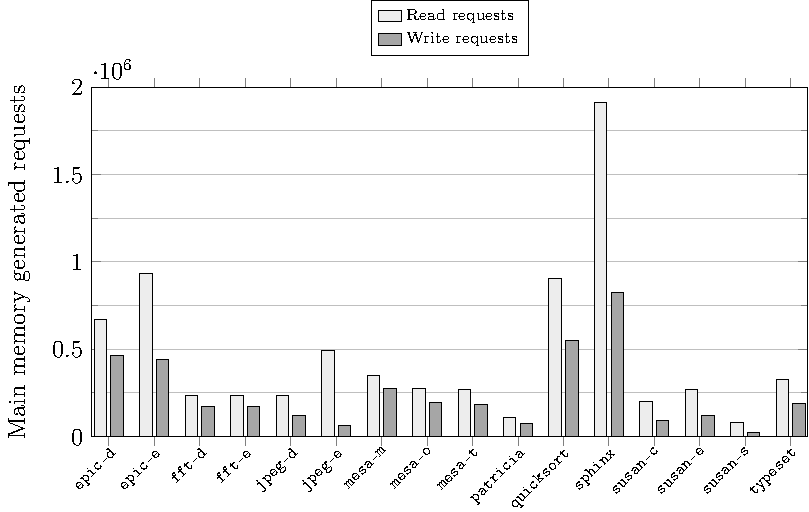
\includegraphics[scale=0.75]{pdfimages/requests-more-50k}
\end{figure}
\end{frame}

\begin{frame}[fragile] \frametitle{Outras funcionalidades}
\begin{itemize}
	\item Códigos
	\begin{itemize}
		\item Pacote listings
	\end{itemize}
\end{itemize}

\begin{figure}[!h]
\begin{lstlisting}[language=C++]
class Coord {
private:
	int x;
	int y;

public:
	Coord(int x, int y){
		this.x = x;
		this.y = y;
	}

	int getX(){ return x; }
	int getY(){ return y; }
}
\end{lstlisting}
\end{figure}
\end{frame}


